%----------------------------------------------------------------------
\section[Canal Youtube]{Canal de YouTube: Ingeniero De Aviones}
%----------------------------------------------------------------------

%----------------------------------------------------------------------
\paragraph{Descripción y objetivo}
%----------------------------------------------------------------------

Tras haber finalizado el simulador con éxito, me dí cuenta de que mucha gente aficionada a la simulación aérea estaba interesada en llevar a cabo la misma tarea con intereses personales, es decir, tener un pequeño simulador en su casa con el que sentirse más cerca de su avión favorito.\\

\begin{wrapfigure}{r}{0.5\linewidth}
	\centering
	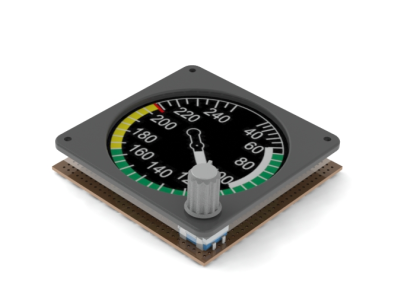
\includegraphics[width=0.5\textwidth]{art1.png}
	\caption*{Gauge para simular un anemómetro}
	\label{labelformat=empty}
\end{wrapfigure}

Sin embargo, muchos aficionados no poseían los conocimientos técnicos por lo que decidí compartir mis ideas en forma de vídeo en la plataforma de YouTube bajo el nombre de 'Ingeniero De Aviones', lo que tuvo una muy buena acogida entre la comunidad aeronáutica.


\paragraph{Primer año de actividad}

Durante el primer año, la temática del canal se centró en la realización de video-tutoriales en los que yo mismo explicaba como diseñar, programar y construir diferentes componentes útiles para la fabricación de cabinas caseras. Durante esta época muchos fueron los que se pusieron en contacto personal conmigo para pedirme ayuda a la hora de llevar a cabo su pequeño sueño de tener un avión en el salón de su casa. Todos los vídeos continúan subidos a la plataforma de YouTube y siguen recibiendo gran cantidad de comentarios en su mayoría positivos.

\paragraph{Segundo año de actividad}

Después de un tiempo, comencé a subir vídeos relacionados con las asignaturas del grado de Ingeniería Aeroespacial (grado que curso). El primer curso titulado "Curso de Mecánica de Fluidos" es el curso de referencia a día de hoy en YouTube para cualquier estudiantes no sólo de Aeronátuica, sino también del resto de Ingenierías. A partir del gran éxito (+20000 reproducciones por vídeo) continúe subiendo contenido de: ecuaciones diferenciales, resistencia de materiales, programación...

\paragraph{Charla "Mi propio simulador de vuelo con Arduino"}

Durante el año 2016, invitado por la asociación "Asrob" de la Universidad Carlos III de Madrid ofrecí una charla en la que mostraba algunos ejemplos básicos para construir un simulador de vuelo sencillo con el famoso microcontrolador.

\begin{figure}[h]
	\centering
	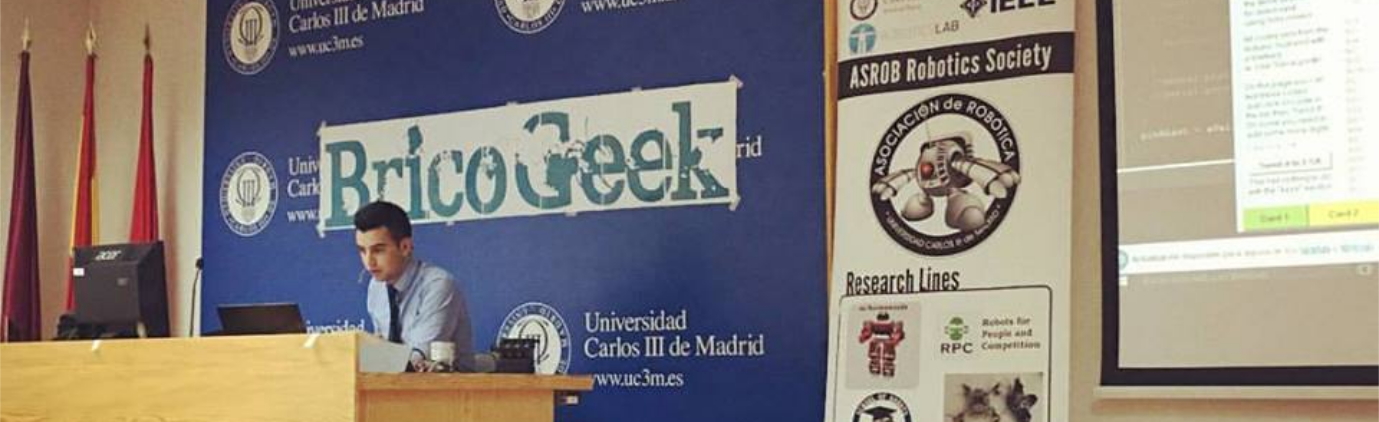
\includegraphics[scale=0.45]{charla.png}
\end{figure}



